\documentclass[a4paper,12pt,oneside]{book}
\usepackage[utf8]{inputenc}
\usepackage{textcomp}
\usepackage[parfill]{parskip} %Se necessatrio non indenta, ma inserisce spazio
\usepackage{graphicx}
\usepackage{hyperref}
\usepackage{amsmath} %To number equations

\usepackage{titling}
\newcommand{\subtitle}[1]{%
 \posttitle{%
 \par\end{center}
 \begin{center}\large#1\end{center}
 \vskip6.5em}%
}

\author{Andrea Onofri and Dario Sacco}
\date{Update: v. 0.99 (2021-12-01), compil. 2021-12-01}
\title{Experimental methods in agriculture}
\subtitle{}


%***************************************************************

%Specific RMarkdown
\usepackage{color}
\usepackage{fancyvrb}
\usepackage{longtable}
\usepackage{booktabs}
\providecommand{\tightlist}{%
  \setlength{\itemsep}{0pt}\setlength{\parskip}{0pt}}
\newcommand{\VerbBar}{|}
\newcommand{\VERB}{\Verb[commandchars=\\\{\}]}
\DefineVerbatimEnvironment{Highlighting}{Verbatim}{commandchars=\\\{\},fontsize=\small}
\usepackage{framed}
%\newenvironment{Shaded}{}{}
\newenvironment{Shaded}{\begin{snugshade}}{\end{snugshade}}
\definecolor{shadecolor}{RGB}{250,248,248}
\newcommand{\KeywordTok}[1]{#1}
\newcommand{\DataTypeTok}[1]{#1}
\newcommand{\DecValTok}[1]{#1}
\newcommand{\BaseNTok}[1]{#1}
\newcommand{\FloatTok}[1]{#1}
\newcommand{\ConstantTok}[1]{#1}
\newcommand{\CharTok}[1]{#1}
\newcommand{\SpecialCharTok}[1]{#1}
\newcommand{\StringTok}[1]{#1}
\newcommand{\VerbatimStringTok}[1]{#1}
\newcommand{\SpecialStringTok}[1]{#1}
\newcommand{\ImportTok}[1]{#1}
\newcommand{\CommentTok}[1]{#1}
\newcommand{\DocumentationTok}[1]{#1}
\newcommand{\AnnotationTok}[1]{#1}
\newcommand{\CommentVarTok}[1]{#1}
\newcommand{\OtherTok}[1]{#1}
\newcommand{\FunctionTok}[1]{#1}
\newcommand{\VariableTok}[1]{#1}
\newcommand{\ControlFlowTok}[1]{#1}
\newcommand{\OperatorTok}[1]{#1}
\newcommand{\BuiltInTok}[1]{#1}
\newcommand{\ExtensionTok}[1]{#1}
\newcommand{\PreprocessorTok}[1]{#1}
\newcommand{\AttributeTok}[1]{#1}
\newcommand{\RegionMarkerTok}[1]{#1}
\newcommand{\InformationTok}[1]{#1}
\newcommand{\WarningTok}[1]{#1}
\newcommand{\AlertTok}[1]{#1}
\newcommand{\ErrorTok}[1]{#1}
\newcommand{\NormalTok}[1]{#1}
% Redefine \includegraphics so that, unless explicit options are
% given, the image width will not exceed the width of the page.
% Images get their normal width if they fit onto the page, but
% are scaled down if they would overflow the margins.

\begin{document}

\maketitle
\tableofcontents

\hypertarget{introduction}{%
\chapter*{Introduction}\label{introduction}}
\addcontentsline{toc}{chapter}{Introduction}

Placeholder

\hypertarget{aims}{%
\section*{Aims}\label{aims}}
\addcontentsline{toc}{section}{Aims}

\hypertarget{how-this-book-is-organised}{%
\section*{How this book is organised}\label{how-this-book-is-organised}}
\addcontentsline{toc}{section}{How this book is organised}

\hypertarget{statistical-software}{%
\section*{Statistical software}\label{statistical-software}}
\addcontentsline{toc}{section}{Statistical software}

\hypertarget{the-authors}{%
\section*{The authors}\label{the-authors}}
\addcontentsline{toc}{section}{The authors}

\hypertarget{science-and-pseudoscience}{%
\chapter{Science and pseudoscience}\label{science-and-pseudoscience}}

Placeholder

\hypertarget{science-needs-data}{%
\section{Science needs data}\label{science-needs-data}}

\hypertarget{not-all-data-support-science}{%
\section{Not all data support science}\label{not-all-data-support-science}}

\hypertarget{good-data-is-based-on-good-methods}{%
\section{Good data is based on good `methods'}\label{good-data-is-based-on-good-methods}}

\hypertarget{the-falsification-principle}{%
\section{The `falsification' principle}\label{the-falsification-principle}}

\hypertarget{trying-to-falsify-a-result}{%
\section{Trying to falsify a result}\label{trying-to-falsify-a-result}}

\hypertarget{the-basic-principles-of-experimental-design}{%
\section{The basic principles of experimental design}\label{the-basic-principles-of-experimental-design}}

\hypertarget{control}{%
\subsection{Control}\label{control}}

\hypertarget{replication}{%
\subsection{Replication}\label{replication}}

\hypertarget{randomisation}{%
\subsection{Randomisation}\label{randomisation}}

\hypertarget{invalid-experiments}{%
\section{Invalid experiments}\label{invalid-experiments}}

\hypertarget{lack-of-good-control}{%
\subsection{Lack of good control}\label{lack-of-good-control}}

\hypertarget{confounding-and-spurious-correlation}{%
\subsection{`Confounding' and spurious correlation}\label{confounding-and-spurious-correlation}}

\hypertarget{lack-of-true-replicates-or-careless-randomisation}{%
\subsection{Lack of true-replicates or careless randomisation}\label{lack-of-true-replicates-or-careless-randomisation}}

\hypertarget{how-can-we-assess-whether-the-data-is-valid}{%
\section{How can we assess whether the data is valid?}\label{how-can-we-assess-whether-the-data-is-valid}}

\hypertarget{conclusions}{%
\section{Conclusions}\label{conclusions}}

\hypertarget{further-readings}{%
\section{Further readings}\label{further-readings}}

\hypertarget{designing-experiments}{%
\chapter{Designing experiments}\label{designing-experiments}}

Placeholder

\hypertarget{the-elements-of-research}{%
\section{The elements of research}\label{the-elements-of-research}}

\hypertarget{hypothesis-and-objectives}{%
\section{Hypothesis and objectives}\label{hypothesis-and-objectives}}

\hypertarget{the-experimental-treatments}{%
\section{The experimental treatments}\label{the-experimental-treatments}}

\hypertarget{factorial-experiments}{%
\subsection{Factorial experiments}\label{factorial-experiments}}

\hypertarget{the-control}{%
\subsection{The control}\label{the-control}}

\hypertarget{the-experimental-units}{%
\section{The experimental units}\label{the-experimental-units}}

\hypertarget{the-allocation-of-treatments}{%
\section{The allocation of treatments}\label{the-allocation-of-treatments}}

\hypertarget{the-variables}{%
\section{The variables}\label{the-variables}}

\hypertarget{nominal-variables}{%
\subsection{Nominal variables}\label{nominal-variables}}

\hypertarget{ordinal-variables}{%
\subsection{Ordinal variables}\label{ordinal-variables}}

\hypertarget{count-and-ratio-variables}{%
\subsection{Count and ratio variables}\label{count-and-ratio-variables}}

\hypertarget{continuous-variables}{%
\subsection{Continuous variables}\label{continuous-variables}}

\hypertarget{sensory-and-visual-assessments}{%
\subsection{Sensory and visual assessments}\label{sensory-and-visual-assessments}}

\hypertarget{setting-up-a-field-experiment}{%
\section{Setting up a field experiment}\label{setting-up-a-field-experiment}}

\hypertarget{selecting-the-field}{%
\subsection{Selecting the field}\label{selecting-the-field}}

\hypertarget{selecting-the-units-within-the-field}{%
\subsection{Selecting the units within the field}\label{selecting-the-units-within-the-field}}

\hypertarget{number-of-replicates}{%
\subsection{Number of replicates}\label{number-of-replicates}}

\hypertarget{the-field-map}{%
\subsection{The field map}\label{the-field-map}}

\hypertarget{the-experimental-lay-out}{%
\subsection{The experimental lay-out}\label{the-experimental-lay-out}}

\hypertarget{completely-randomised-design-cr}{%
\subsubsection{Completely randomised design (CR)}\label{completely-randomised-design-cr}}

\hypertarget{randomised-complete-block-design-rcbd}{%
\subsubsection{Randomised complete block design (RCBD)}\label{randomised-complete-block-design-rcbd}}

\hypertarget{latin-square-design}{%
\subsubsection{Latin square design}\label{latin-square-design}}

\hypertarget{split-plot-and-strip-plot-designs}{%
\subsubsection{Split-plot and strip-plot designs}\label{split-plot-and-strip-plot-designs}}

\hypertarget{conclusions-1}{%
\section{Conclusions}\label{conclusions-1}}

\hypertarget{further-readings-1}{%
\section{Further readings}\label{further-readings-1}}

\hypertarget{describing-the-observations}{%
\chapter{Describing the observations}\label{describing-the-observations}}

Placeholder

\hypertarget{quantitative-data}{%
\section{Quantitative data}\label{quantitative-data}}

\hypertarget{statistics-of-location}{%
\subsection{Statistics of location}\label{statistics-of-location}}

\hypertarget{statistics-of-spread}{%
\subsection{Statistics of spread}\label{statistics-of-spread}}

\hypertarget{summing-the-uncertainty}{%
\subsection{Summing the uncertainty}\label{summing-the-uncertainty}}

\hypertarget{relationship-between-quantitative-variables}{%
\subsection{Relationship between quantitative variables}\label{relationship-between-quantitative-variables}}

\hypertarget{nominal-data}{%
\section{Nominal data}\label{nominal-data}}

\hypertarget{distributions-of-frequencies}{%
\subsection{Distributions of frequencies}\label{distributions-of-frequencies}}

\hypertarget{descriptive-stats-for-distributions-of-frequencies}{%
\subsection{Descriptive stats for distributions of frequencies}\label{descriptive-stats-for-distributions-of-frequencies}}

\hypertarget{contingency-tables}{%
\subsection{Contingency tables}\label{contingency-tables}}

\hypertarget{independence}{%
\subsection{Independence}\label{independence}}

\hypertarget{descriptive-stats-with-r}{%
\section{Descriptive stats with R}\label{descriptive-stats-with-r}}

\hypertarget{graphical-representations}{%
\section{Graphical representations}\label{graphical-representations}}

\hypertarget{further-reading}{%
\section{Further reading}\label{further-reading}}

\hypertarget{modeling-the-experimental-data}{%
\chapter{Modeling the experimental data}\label{modeling-the-experimental-data}}

Placeholder

\hypertarget{deterministic-models}{%
\section{Deterministic models}\label{deterministic-models}}

\hypertarget{stochastic-models}{%
\section{Stochastic models}\label{stochastic-models}}

\hypertarget{probability-functions}{%
\subsection{Probability functions}\label{probability-functions}}

\hypertarget{density-functions}{%
\subsection{Density functions}\label{density-functions}}

\hypertarget{the-gaussian-pdf-and-cdf}{%
\subsection{The Gaussian PDF and CDF}\label{the-gaussian-pdf-and-cdf}}

\hypertarget{a-model-with-two-components}{%
\section{A model with two components}\label{a-model-with-two-components}}

\hypertarget{and-so-what}{%
\section{And so what?}\label{and-so-what}}

\hypertarget{monte-carlo-methods-to-simulate-an-experiment}{%
\section{Monte Carlo methods to simulate an experiment}\label{monte-carlo-methods-to-simulate-an-experiment}}

\hypertarget{data-analysis-and-model-fitting}{%
\section{Data analysis and model fitting}\label{data-analysis-and-model-fitting}}

\hypertarget{some-words-of-warning}{%
\section{Some words of warning}\label{some-words-of-warning}}

\hypertarget{further-readings-2}{%
\section{Further readings}\label{further-readings-2}}

\hypertarget{estimation-of-model-parameters}{%
\chapter{Estimation of model parameters}\label{estimation-of-model-parameters}}

Placeholder

\hypertarget{example-1-a-concentration-value}{%
\section{Example 1: a concentration value}\label{example-1-a-concentration-value}}

\hypertarget{the-empirical-sampling-distribution}{%
\subsection{The empirical sampling distribution}\label{the-empirical-sampling-distribution}}

\hypertarget{a-theoretical-sampling-distribution}{%
\subsection{A theoretical sampling distribution}\label{a-theoretical-sampling-distribution}}

\hypertarget{the-frequentist-confidence-interval}{%
\subsection{The frequentist confidence interval}\label{the-frequentist-confidence-interval}}

\hypertarget{example-2-a-proportion}{%
\section{Example 2: a proportion}\label{example-2-a-proportion}}

\hypertarget{conclusions-2}{%
\section{Conclusions}\label{conclusions-2}}

\hypertarget{further-readings-3}{%
\section{Further readings}\label{further-readings-3}}

\hypertarget{making-decisions-under-uncertainty}{%
\chapter{Making Decisions under uncertainty}\label{making-decisions-under-uncertainty}}

Placeholder

\hypertarget{comparing-sample-means-the-students-t-test}{%
\section{Comparing sample means: the Student's t-test}\label{comparing-sample-means-the-students-t-test}}

\hypertarget{the-dataset}{%
\subsection{The dataset}\label{the-dataset}}

\hypertarget{monte-carlo-simulation}{%
\subsection{Monte Carlo simulation}\label{monte-carlo-simulation}}

\hypertarget{a-formal-solution}{%
\subsection{A formal solution}\label{a-formal-solution}}

\hypertarget{the-t-test-with-r}{%
\subsection{The t test with R}\label{the-t-test-with-r}}

\hypertarget{comparing-proportions-the-chi2-test}{%
\section{\texorpdfstring{Comparing proportions: the \(\chi^2\) test}{Comparing proportions: the \textbackslash chi\^{}2 test}}\label{comparing-proportions-the-chi2-test}}

\hypertarget{correct-interpretation-of-the-p-value}{%
\section{Correct interpretation of the P-value}\label{correct-interpretation-of-the-p-value}}

\hypertarget{conclusions-3}{%
\section{Conclusions}\label{conclusions-3}}

\hypertarget{further-readings-4}{%
\section{Further readings}\label{further-readings-4}}

\hypertarget{one-way-anova-models}{%
\chapter{One-way ANOVA models}\label{one-way-anova-models}}

Placeholder

\hypertarget{comparing-herbicides-in-a-pot-experiment}{%
\section{Comparing herbicides in a pot-experiment}\label{comparing-herbicides-in-a-pot-experiment}}

\hypertarget{data-description}{%
\section{Data description}\label{data-description}}

\hypertarget{model-definition}{%
\section{Model definition}\label{model-definition}}

\hypertarget{parameterisation}{%
\subsection{Parameterisation}\label{parameterisation}}

\hypertarget{treatment-constraint}{%
\subsection{Treatment constraint}\label{treatment-constraint}}

\hypertarget{sum-to-zero-constraint}{%
\subsection{Sum-to-zero constraint}\label{sum-to-zero-constraint}}

\hypertarget{basic-assumptions}{%
\section{Basic assumptions}\label{basic-assumptions}}

\hypertarget{fitting-anova-models-by-hand}{%
\section{Fitting ANOVA models by hand}\label{fitting-anova-models-by-hand}}

\hypertarget{parameter-estimation}{%
\subsection{Parameter estimation}\label{parameter-estimation}}

\hypertarget{residuals}{%
\subsection{Residuals}\label{residuals}}

\hypertarget{standard-deviation-sigma}{%
\subsection{\texorpdfstring{Standard deviation \(\sigma\)}{Standard deviation \textbackslash sigma}}\label{standard-deviation-sigma}}

\hypertarget{sem-and-sed}{%
\subsection{SEM and SED}\label{sem-and-sed}}

\hypertarget{variance-partitioning}{%
\subsection{Variance partitioning}\label{variance-partitioning}}

\hypertarget{hypothesis-testing}{%
\subsection{Hypothesis testing}\label{hypothesis-testing}}

\hypertarget{fitting-anova-models-with-r}{%
\section{Fitting ANOVA models with R}\label{fitting-anova-models-with-r}}

\hypertarget{expected-marginal-means}{%
\section{Expected marginal means}\label{expected-marginal-means}}

\hypertarget{conclusions-4}{%
\section{Conclusions}\label{conclusions-4}}

\hypertarget{further-readings-5}{%
\section{Further readings}\label{further-readings-5}}

\hypertarget{checking-for-the-basic-assumptions}{%
\chapter{Checking for the basic assumptions}\label{checking-for-the-basic-assumptions}}

Placeholder

\hypertarget{outlying-observations}{%
\section{Outlying observations}\label{outlying-observations}}

\hypertarget{the-inspection-of-residuals}{%
\section{The inspection of residuals}\label{the-inspection-of-residuals}}

\hypertarget{plot-of-residuals-against-expected-values}{%
\subsection{Plot of residuals against expected values}\label{plot-of-residuals-against-expected-values}}

\hypertarget{qq-plot}{%
\subsection{QQ-plot}\label{qq-plot}}

\hypertarget{formal-hypotesis-testing}{%
\section{Formal hypotesis testing}\label{formal-hypotesis-testing}}

\hypertarget{what-do-we-do-in-practice}{%
\section{What do we do, in practice?}\label{what-do-we-do-in-practice}}

\hypertarget{correcting-measures}{%
\section{Correcting measures}\label{correcting-measures}}

\hypertarget{removing-outliers}{%
\subsection{Removing outliers}\label{removing-outliers}}

\hypertarget{stabilising-transformations}{%
\subsection{Stabilising transformations}\label{stabilising-transformations}}

\hypertarget{examples-with-r}{%
\section{Examples with R}\label{examples-with-r}}

\hypertarget{example-1}{%
\section{Example 1}\label{example-1}}

\hypertarget{example-2}{%
\section{Example 2}\label{example-2}}

\hypertarget{other-possible-approaches}{%
\section{Other possible approaches}\label{other-possible-approaches}}

\hypertarget{further-readings-6}{%
\section{Further readings}\label{further-readings-6}}

\hypertarget{contrasts-and-multiple-comparison-testing}{%
\chapter{Contrasts and multiple comparison testing}\label{contrasts-and-multiple-comparison-testing}}

Placeholder

\hypertarget{back-to-the-mixture-example}{%
\section{Back to the `mixture' example}\label{back-to-the-mixture-example}}

\hypertarget{linear-contrasts}{%
\section{Linear contrasts}\label{linear-contrasts}}

\hypertarget{the-variance-of-contrasts}{%
\subsection{The variance of contrasts}\label{the-variance-of-contrasts}}

\hypertarget{testing-linear-contrasts-with-r}{%
\subsection{Testing linear contrasts with R}\label{testing-linear-contrasts-with-r}}

\hypertarget{pairwise-comparisons}{%
\section{Pairwise comparisons}\label{pairwise-comparisons}}

\hypertarget{letter-display}{%
\section{Letter display}\label{letter-display}}

\hypertarget{multiplicity-correction}{%
\section{Multiplicity correction}\label{multiplicity-correction}}

\hypertarget{multiple-comparisons-with-transformed-data}{%
\section{Multiple comparisons with transformed data}\label{multiple-comparisons-with-transformed-data}}

\hypertarget{what-about-the-traditional-mcps}{%
\section{What about the traditional MCPs?}\label{what-about-the-traditional-mcps}}

\hypertarget{some-practical-suggestions}{%
\section{Some practical suggestions}\label{some-practical-suggestions}}

\hypertarget{further-readings-7}{%
\section{Further readings}\label{further-readings-7}}

\hypertarget{multi-way-anova-models}{%
\chapter{Multi-way ANOVA models}\label{multi-way-anova-models}}

Placeholder

\hypertarget{motivating-example-a-genotype-experiment-in-blocks}{%
\section{Motivating example: a genotype experiment in blocks}\label{motivating-example-a-genotype-experiment-in-blocks}}

\hypertarget{model-definition-1}{%
\section{Model definition}\label{model-definition-1}}

\hypertarget{model-fitting-by-hand}{%
\section{Model fitting by hand}\label{model-fitting-by-hand}}

\hypertarget{model-fitting-with-r}{%
\section{Model fitting with R}\label{model-fitting-with-r}}

\hypertarget{model-checking}{%
\subsection{Model checking}\label{model-checking}}

\hypertarget{variance-partitioning-1}{%
\subsection{Variance partitioning}\label{variance-partitioning-1}}

\hypertarget{another-example-comparing-working-protocols}{%
\section{Another example: comparing working protocols}\label{another-example-comparing-working-protocols}}

\hypertarget{multi-way-anova-models-with-interactions}{%
\chapter{Multi-way ANOVA models with interactions}\label{multi-way-anova-models-with-interactions}}

Placeholder

\hypertarget{the-interaction-concept}{%
\section{The `interaction' concept}\label{the-interaction-concept}}

\hypertarget{genotype-by-n-interactions}{%
\section{Genotype by N interactions}\label{genotype-by-n-interactions}}

\hypertarget{model-definition-2}{%
\subsection{Model definition}\label{model-definition-2}}

\hypertarget{model-fitting-by-hand-1}{%
\subsection{Model fitting by hand}\label{model-fitting-by-hand-1}}

\hypertarget{model-fitting-with-r-1}{%
\subsection{Model fitting with R}\label{model-fitting-with-r-1}}

\hypertarget{inferences-and-standard-errors}{%
\subsection{Inferences and standard errors}\label{inferences-and-standard-errors}}

\hypertarget{expected-marginal-means-1}{%
\subsection{Expected marginal means}\label{expected-marginal-means-1}}

\hypertarget{nested-effects-maize-crosses}{%
\section{Nested effects: maize crosses}\label{nested-effects-maize-crosses}}

\hypertarget{model-definition-3}{%
\subsection{Model definition}\label{model-definition-3}}

\hypertarget{parameter-estimation-1}{%
\subsection{Parameter estimation}\label{parameter-estimation-1}}

\hypertarget{further-readings-8}{%
\section{Further readings}\label{further-readings-8}}

\hypertarget{plots-of-different-sizes}{%
\chapter{Plots of different sizes}\label{plots-of-different-sizes}}

Placeholder

\hypertarget{example-1-a-split-plot-experiment}{%
\section{Example 1: a split-plot experiment}\label{example-1-a-split-plot-experiment}}

\hypertarget{model-definition-4}{%
\subsection{Model definition}\label{model-definition-4}}

\hypertarget{model-fitting-with-r-2}{%
\subsection{Model fitting with R}\label{model-fitting-with-r-2}}

\hypertarget{example-2-a-strip-plot-design}{%
\section{Example 2: a strip-plot design}\label{example-2-a-strip-plot-design}}

\hypertarget{model-definition-5}{%
\subsection{Model definition}\label{model-definition-5}}

\hypertarget{model-fitting-with-r-3}{%
\subsection{Model fitting with R}\label{model-fitting-with-r-3}}

\hypertarget{further-readings-9}{%
\section{Further readings}\label{further-readings-9}}

\hypertarget{simple-linear-regression}{%
\chapter{Simple linear regression}\label{simple-linear-regression}}

Placeholder

\hypertarget{case-study-n-fertilisation-in-wheat}{%
\section{Case-study: N fertilisation in wheat}\label{case-study-n-fertilisation-in-wheat}}

\hypertarget{preliminary-analysis}{%
\section{Preliminary analysis}\label{preliminary-analysis}}

\hypertarget{definition-of-a-linear-model}{%
\section{Definition of a linear model}\label{definition-of-a-linear-model}}

\hypertarget{parameter-estimation-2}{%
\section{Parameter estimation}\label{parameter-estimation-2}}

\hypertarget{goodness-of-fit}{%
\section{Goodness of fit}\label{goodness-of-fit}}

\hypertarget{graphical-evaluation}{%
\subsection{Graphical evaluation}\label{graphical-evaluation}}

\hypertarget{standard-errors-for-parameter-estimates}{%
\subsection{Standard errors for parameter estimates}\label{standard-errors-for-parameter-estimates}}

\hypertarget{f-test-for-lack-of-fit}{%
\subsection{F test for lack of fit}\label{f-test-for-lack-of-fit}}

\hypertarget{f-test-for-goodness-of-fit-and-coefficient-of-determination}{%
\subsection{F test for goodness of fit and coefficient of determination}\label{f-test-for-goodness-of-fit-and-coefficient-of-determination}}

\hypertarget{making-predictions}{%
\section{Making predictions}\label{making-predictions}}

\hypertarget{further-readings-10}{%
\section{Further readings}\label{further-readings-10}}

\hypertarget{nonlinear-regression}{%
\chapter{Nonlinear regression}\label{nonlinear-regression}}

Biological processes, very rarely follow linear trends. Just think about how a crop grows, or responds to increasing doses of fertilisers/xenobiotics. Or, think about how an herbicide degrades in the soil, or about the germination pattern of a seed population. It is very easy to realise that curvilinear trends, asymptotes and/or inflection points are far more common, in nature. In practice, linear equations in biology are nothing more than a quick way to approximate a response over a very narrow range of the independent variable.

Therefore, we need to be able to fit simple nonlinear models to our experimental data. In this Chapter, we will see how to do this, starting from a simple, but realistic example.

\hypertarget{case-study-a-degradation-curve}{%
\section{Case-study: a degradation curve}\label{case-study-a-degradation-curve}}

A soil was enriched with the herbicide metamitron, up to a concentration of 100 ng g\textsuperscript{1}. It was put in 24 aluminium containers, inside a climatic chamber at 20°C. Three containers were randomly selected in eight different times and the residual concentration of metamitron was measured. The observed data are available in the `degradation.csv' file, in an external repository. First of all we load and inspect the data.

\vspace{12pt}

\begin{Shaded}
\begin{Highlighting}[]
\NormalTok{fileName }\OtherTok{\textless{}{-}} \StringTok{"https://www.casaonofri.it/\_datasets/degradation.csv"}
\NormalTok{dataset }\OtherTok{\textless{}{-}} \FunctionTok{read.csv}\NormalTok{(fileName, }\AttributeTok{header=}\NormalTok{T)}
\FunctionTok{head}\NormalTok{(dataset, }\DecValTok{10}\NormalTok{)}
\end{Highlighting}
\end{Shaded}

\begin{verbatim}
##    Time   Conc
## 1     0  96.40
## 2    10  46.30
## 3    20  21.20
## 4    30  17.89
## 5    40  10.10
## 6    50   6.90
## 7    60   3.50
## 8    70   1.90
## 9     0 102.30
## 10   10  49.20
\end{verbatim}

It is always very useful to take a look at the observed data, by plotting the response against the predictor (Figure \ref{fig:figName150}); we see that the trend is curvilinear, which rules out the use of simple linear regression.

In order to build a nonlinear regression model, we can use the general form introduced in Chapter 4, that is:

\[Y_i = f(X_i, \theta) + \varepsilon_i\]

where \(X\) is the time, \(Y\) is the concentration, \(f\) is a nonlinear function, \(\theta\) is the set of model parameters and \(\varepsilon\) are the residuals, assumed as independent, gaussian and homoscedastic.

\begin{figure}

{\centering 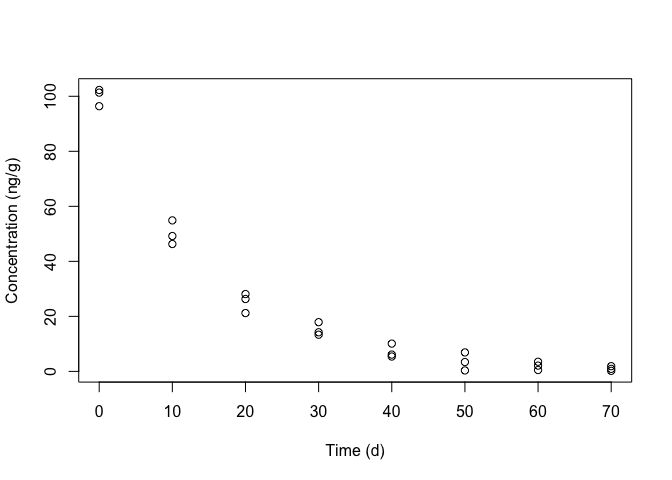
\includegraphics[width=0.9\linewidth]{_main_files/figure-latex/figName150-1} 

}

\caption{Degradation of metamitron in soil}\label{fig:figName150}
\end{figure}

\hypertarget{model-selection}{%
\section{Model selection}\label{model-selection}}

The first task is to select a function \(f\) that matches the observed response shape. You can find full detail elsewhere (go to \href{https://www.statforbiology.com/2020/stat_nls_usefulfunctions/}{this link}). For now, we can look at Figure \ref{fig:figName151}, where we have displayed the shapes of some useful functions for nonlinear regression analysis in agricultural studies. We distinguish:

\begin{enumerate}
\def\labelenumi{\arabic{enumi}.}
\tightlist
\item
  Convex/concave shapes (e.g., quadratic polynomial, exponential growth/decay, asymptotic growth, power curve and rectangular hyperbola)
\item
  Sigmoidal shapes (e.g., logistic growth, Gompertz growth and log-logistic dose-response)
\item
  Curves with maxima/minima (e.g., Bragg's function)
\end{enumerate}

In the above list, the quadratic polynomial is a curvilinear model, but it is linear in the parameters and, therefore, it should have been better included in the previous Chapter about linear regression. However, we decided to include it here, considering its concave shape.

\begin{figure}

{\centering 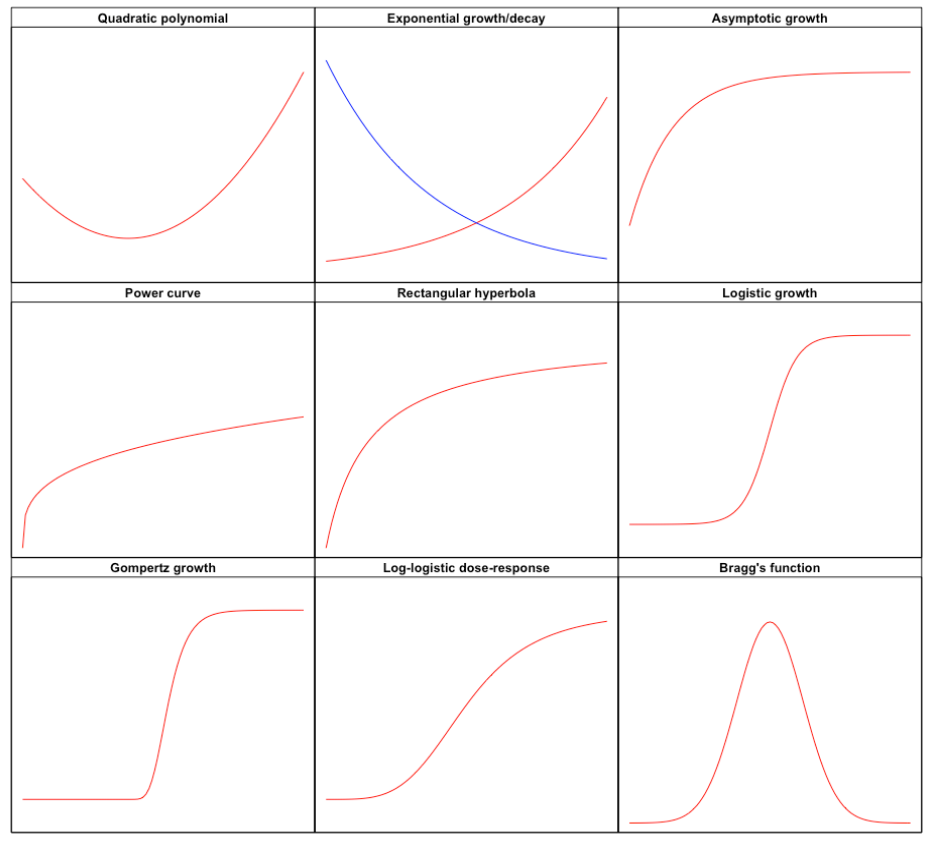
\includegraphics[width=0.95\linewidth]{_images/nonLinearCurves} 

}

\caption{The shapes of the most important functions}\label{fig:figName151}
\end{figure}

Behind each of the above shapes, there is a mathematical function, which is shown in Figure \ref{fig:figName151bis} ).

\begin{figure}

{\centering 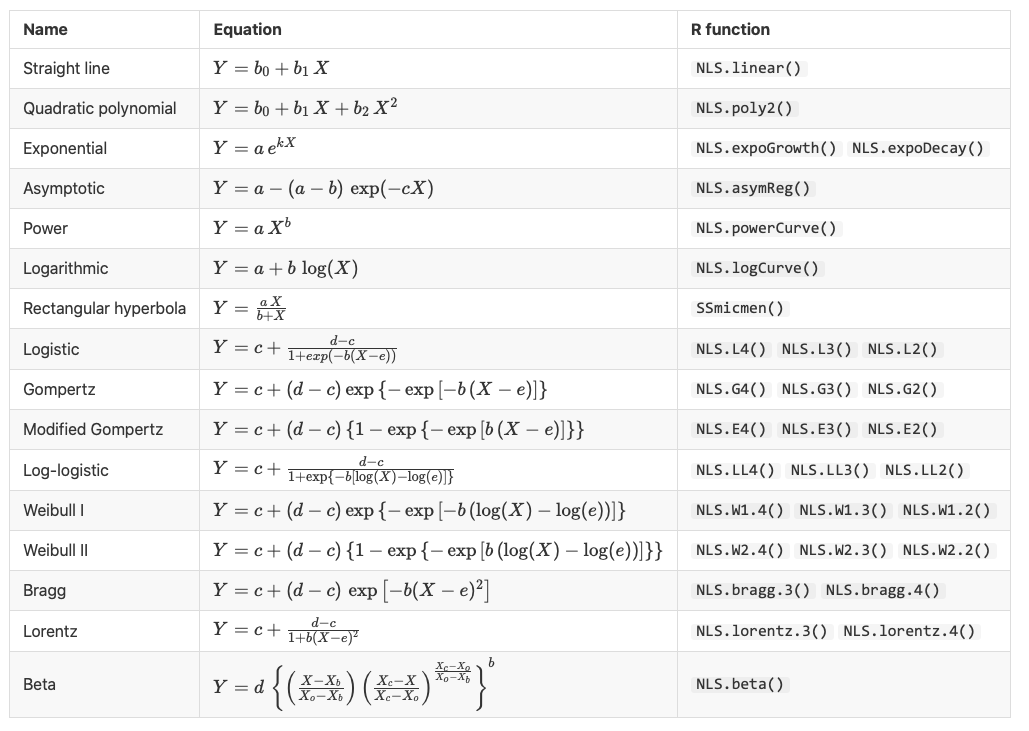
\includegraphics[width=0.95\linewidth]{_images/nonLinearEquations} 

}

\caption{Some useful functions for nonlinear regression analysis (equation and R function).}\label{fig:figName151bis}
\end{figure}

For the dataset under study, considering the shapes in Figure \ref{fig:figName151} and, above all, considering the available literature information, we select an exponential decay equation, with the following form (see also Fig. \ref{fig:figName151bis} ):

\[Y_i = a \, e^{-k \,X_i} + \varepsilon_i\]

where \(Y\) is the concentration at time \(X\), \(a\) is the initial metamitron concentration and \(k\) is the constant degradation rate.

\hypertarget{parameter-estimation-3}{%
\section{Parameter estimation}\label{parameter-estimation-3}}

Now, we have to obtain the least squares estimates of the parameters \(a\) and \(k\). Unfortunately, with nonlinear regression, the least squares problem has no closed form solution and, therefore, we need to tackle the estimation problem in a different way. In general, there are three possibilities

\begin{enumerate}
\def\labelenumi{\arabic{enumi}.}
\tightlist
\item
  linearise the nonlinear function;
\item
  approximate the nonlinear function by using a polynomial;
\item
  use numerical methods for the minimisation.
\end{enumerate}

Let's see advantages and disadvantages of all methods.

\hypertarget{linearisation}{%
\subsection{Linearisation}\label{linearisation}}

In some cases, we can modify the function to make it linear. In this case, we can take the logarithm of both sides and define the following equation:

\[ \log(Y) = \log(A) - k \, X \]

which is, indeed, linear. Therefore, we can take the logarithms of the concentrations and fit a linear model, by using the \texttt{lm()} function:

\vspace{12pt}

\begin{Shaded}
\begin{Highlighting}[]
\NormalTok{mod }\OtherTok{\textless{}{-}} \FunctionTok{lm}\NormalTok{(}\FunctionTok{log}\NormalTok{(Conc) }\SpecialCharTok{\textasciitilde{}}\NormalTok{ Time, }\AttributeTok{data=}\NormalTok{dataset)}
\FunctionTok{summary}\NormalTok{(mod)}
\end{Highlighting}
\end{Shaded}

\begin{verbatim}
## 
## Call:
## lm(formula = log(Conc) ~ Time, data = dataset)
## 
## Residuals:
##      Min       1Q   Median       3Q      Max 
## -2.11738 -0.09583  0.05336  0.31166  1.01243 
## 
## Coefficients:
##              Estimate Std. Error t value Pr(>|t|)    
## (Intercept)  4.662874   0.257325   18.12 1.04e-14 ***
## Time        -0.071906   0.006151  -11.69 6.56e-11 ***
## ---
## Signif. codes:  
## 0 '***' 0.001 '**' 0.01 '*' 0.05 '.' 0.1 ' ' 1
## 
## Residual standard error: 0.6905 on 22 degrees of freedom
## Multiple R-squared:  0.8613, Adjusted R-squared:  0.855 
## F-statistic: 136.6 on 1 and 22 DF,  p-value: 6.564e-11
\end{verbatim}

We see that the slope has a negative sign (the line is decreasing) and the intercept is not the initial concentration value, but its logarithm.

The advantage of this process is that the calculations are very easily performed with every spreadsheet or simple calculator. However, we need to check that the basic assumptions of normal and homoscedastic residuals hold in the logarithmic scale. We do this in the following box.

\begin{Shaded}
\begin{Highlighting}[]
\FunctionTok{par}\NormalTok{(}\AttributeTok{mfrow =} \FunctionTok{c}\NormalTok{(}\DecValTok{1}\NormalTok{,}\DecValTok{2}\NormalTok{))}
\FunctionTok{plot}\NormalTok{(mod, }\AttributeTok{which =} \DecValTok{1}\NormalTok{)}
\FunctionTok{plot}\NormalTok{(mod, }\AttributeTok{which =} \DecValTok{2}\NormalTok{)}
\end{Highlighting}
\end{Shaded}

\begin{figure}

{\centering 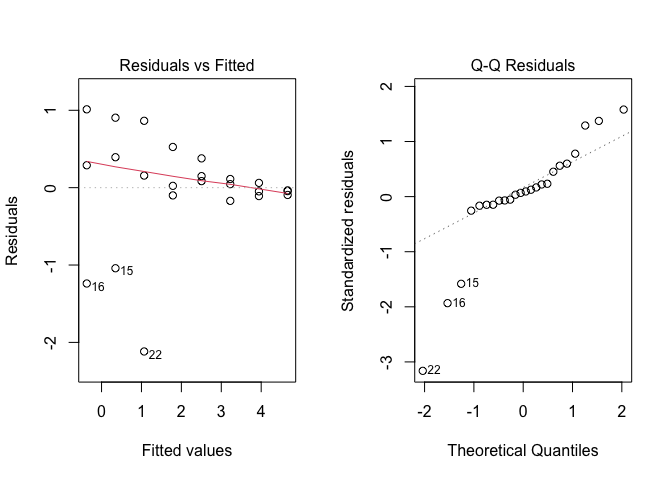
\includegraphics[width=0.9\linewidth]{_main_files/figure-latex/figName152-1} 

}

\caption{Graphical analyses of residuals for nonlinear regression with linearisation of the mean function}\label{fig:figName152}
\end{figure}

The plots show dramatic deviations from homoscedasticity (Figure \ref{fig:figName152} ), which rule out the use of the linearisation method. Please, consider that this conclusion is specific to our dataset, while, in general, the linearisation method can be successfully used, whenever the basic assumptions for linear models appear to hold for the transformed response.

\hypertarget{approximation-with-a-polynomial-function}{%
\subsection{Approximation with a polynomial function}\label{approximation-with-a-polynomial-function}}

In some other cases, a curvilinear shape can be approximated by using a polynomial equation, that is, indeed, linear in the parameters. In our example, we could think of the descending part of a second order polynomial (see Figure \ref{fig:figName152}) and, thus, we fit this model by the usual \texttt{lm()} function:

\begin{Shaded}
\begin{Highlighting}[]
\NormalTok{mod2 }\OtherTok{\textless{}{-}} \FunctionTok{lm}\NormalTok{(Conc }\SpecialCharTok{\textasciitilde{}}\NormalTok{ Time }\SpecialCharTok{+} \FunctionTok{I}\NormalTok{(Time}\SpecialCharTok{\^{}}\DecValTok{2}\NormalTok{), }\AttributeTok{data=}\NormalTok{dataset)}
\NormalTok{pred }\OtherTok{\textless{}{-}} \FunctionTok{predict}\NormalTok{(mod2, }\AttributeTok{newdata =} \FunctionTok{data.frame}\NormalTok{(}\AttributeTok{Time =} \FunctionTok{seq}\NormalTok{(}\DecValTok{0}\NormalTok{, }\DecValTok{70}\NormalTok{, }\AttributeTok{by =} \FloatTok{0.1}\NormalTok{)))}
\FunctionTok{plot}\NormalTok{(Conc }\SpecialCharTok{\textasciitilde{}}\NormalTok{ Time, }\AttributeTok{data=}\NormalTok{dataset)}
\FunctionTok{lines}\NormalTok{(pred }\SpecialCharTok{\textasciitilde{}} \FunctionTok{seq}\NormalTok{(}\DecValTok{0}\NormalTok{, }\DecValTok{70}\NormalTok{, }\AttributeTok{by =} \FloatTok{0.1}\NormalTok{), }\AttributeTok{col =} \StringTok{"red"}\NormalTok{)}
\end{Highlighting}
\end{Shaded}

\begin{figure}

{\centering 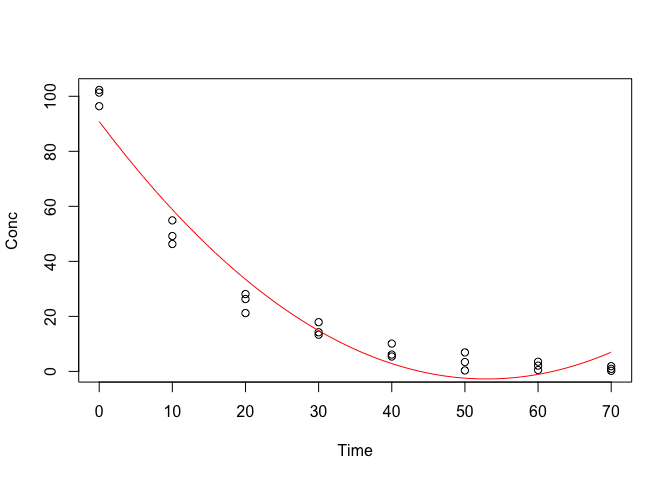
\includegraphics[width=0.9\linewidth]{_main_files/figure-latex/figName153-1} 

}

\caption{Approximating a degradation kinetic by using a second order polynomial}\label{fig:figName153}
\end{figure}

We see that the approximation is good up to 40 days after the beginning of the experiment. Later on, the fitted function appears to deviate from the observed pattern, depicting an unrealistic concentration increase from 55 days onwards (Figure \ref{fig:figName153}). Clearly, the use of polynomials may be useful in some other instances, but it not a suitable solution for this case.

\hypertarget{nonlinear-least-squares}{%
\subsection{Nonlinear least squares}\label{nonlinear-least-squares}}

The third possibility consists of using nonlinear least squares, based on the Gauss-Newton iterative algorithm. We need to provide reasonable initial estimates of model parameters and the algorithm updates them, iteratively, until it converges on the approximate least squares solution. Nowadays, thanks to the advent of modern computers, nonlinear least squares have become the most widespread nonlinear regression method, providing very good approximations for most practical needs.

\hypertarget{nonlinear-regression-with-r}{%
\section{Nonlinear regression with R}\label{nonlinear-regression-with-r}}

Considering the base R installation, nonlinear least squares regression is implemented in the \texttt{nls()} function. The syntax is very similar to that of the \texttt{lm()} function, although we need to provide reasonable initial values for model parameters. In this case, obtaining such values is relatively easy: \(a\) is the initial concentration and, by looking at the data, we can set this value to 100. The parameter \(k\) is the constant degradation rate, i.e.~the percentage daily reduction in concentration; we see that the concentration drops by 50\% in ten days, thus we could assume that there is a daily 5\% drop (k = 0.05). With such an information, we fit the model, as shown in the box below.

\begin{Shaded}
\begin{Highlighting}[]
\NormalTok{modNlin }\OtherTok{\textless{}{-}} \FunctionTok{nls}\NormalTok{(Conc }\SpecialCharTok{\textasciitilde{}}\NormalTok{ A}\SpecialCharTok{*}\FunctionTok{exp}\NormalTok{(}\SpecialCharTok{{-}}\NormalTok{k}\SpecialCharTok{*}\NormalTok{Time), }
               \AttributeTok{start=}\FunctionTok{list}\NormalTok{(}\AttributeTok{A=}\DecValTok{100}\NormalTok{, }\AttributeTok{k=}\FloatTok{0.05}\NormalTok{), }
               \AttributeTok{data =}\NormalTok{ dataset)}
\FunctionTok{summary}\NormalTok{(modNlin)}
\end{Highlighting}
\end{Shaded}

\begin{verbatim}
## 
## Formula: Conc ~ A * exp(-k * Time)
## 
## Parameters:
##    Estimate Std. Error t value Pr(>|t|)    
## A 99.634902   1.461047   68.19   <2e-16 ***
## k  0.067039   0.001887   35.53   <2e-16 ***
## ---
## Signif. codes:  
## 0 '***' 0.001 '**' 0.01 '*' 0.05 '.' 0.1 ' ' 1
## 
## Residual standard error: 2.621 on 22 degrees of freedom
## 
## Number of iterations to convergence: 5 
## Achieved convergence tolerance: 4.33e-07
\end{verbatim}

Instead of coding the mean model from the scratch, we can use one of the available self-starting functions (Fig. \ref{fig:figName151bis} ), which are associated to self-starting routines. This is very useful, as the self-starting functions do not need initial estimates and, thus, we are free from the task of providing them, which is rather difficult for beginners. Indeed, if our initial guesses are not close enough to least squares estimates, the algorithm may freeze during the estimation process and may not reach convergence. Self-starting functions are available within the `aomisc' which needs to be installed from github prior to fitting the model.

\begin{Shaded}
\begin{Highlighting}[]
\CommentTok{\# Installation is required only once}
\CommentTok{\# library(devtools)}
\CommentTok{\# install\_github("onofriandreapg/aomisc")}
\FunctionTok{library}\NormalTok{(aomisc)}
\NormalTok{modNlin2 }\OtherTok{\textless{}{-}} \FunctionTok{nls}\NormalTok{(Conc }\SpecialCharTok{\textasciitilde{}} \FunctionTok{NLS.expoDecay}\NormalTok{(Time, a, k),}
               \AttributeTok{data =}\NormalTok{ dataset)}
\end{Highlighting}
\end{Shaded}

\hypertarget{checking-the-model}{%
\section{Checking the model}\label{checking-the-model}}

While the estimation of model parameters is performed by using numerical methods, checking a fitted model is done by using the very same methods as shown for simple linear regression, with slight differences. In the following section we will show some of the R methods for nonlinear models, which can be used on `nls' objects.

\hypertarget{graphical-analyses-of-residuals}{%
\subsection{Graphical analyses of residuals}\label{graphical-analyses-of-residuals}}

First of all, we check the basic assumptions of normality and homoscedasticity of model residuals, by the usual diagnostic plots. We can us the \texttt{plotnls()} function, as available in the `aomisc' package.

\begin{Shaded}
\begin{Highlighting}[]
\FunctionTok{par}\NormalTok{(}\AttributeTok{mfrow=}\FunctionTok{c}\NormalTok{(}\DecValTok{1}\NormalTok{,}\DecValTok{2}\NormalTok{))}
\FunctionTok{plotnls}\NormalTok{(modNlin, }\AttributeTok{which =} \DecValTok{1}\NormalTok{)}
\FunctionTok{plotnls}\NormalTok{(modNlin, }\AttributeTok{which =} \DecValTok{2}\NormalTok{)}
\end{Highlighting}
\end{Shaded}

\begin{figure}

{\centering 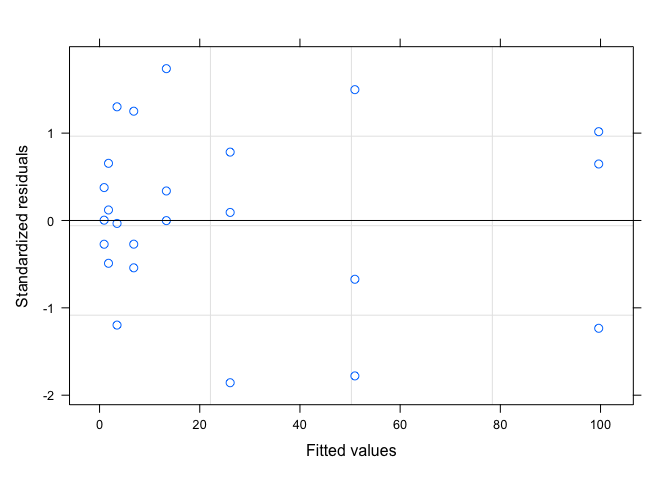
\includegraphics[width=0.9\linewidth]{_main_files/figure-latex/figName154-1} 

}

\caption{Graphical analyses of residuals relating to the degradation of metamitron in soil.}\label{fig:figName154}
\end{figure}

Figure \ref{fig:figName154} does not show any visible deviations and, thus, we proceed to plotting the observed data along with model predictions (Figure \ref{fig:figName155}), e.g., by using the \texttt{plotnls()} function, in the `aomisc' package.

\begin{Shaded}
\begin{Highlighting}[]
\FunctionTok{plotnls}\NormalTok{(modNlin, }\AttributeTok{type =} \StringTok{"means"}\NormalTok{,}
        \AttributeTok{xlab =} \StringTok{"Time (d)"}\NormalTok{, }\AttributeTok{ylab =} \StringTok{"Concentration (ng/g)"}\NormalTok{)}
\end{Highlighting}
\end{Shaded}

\begin{figure}

{\centering 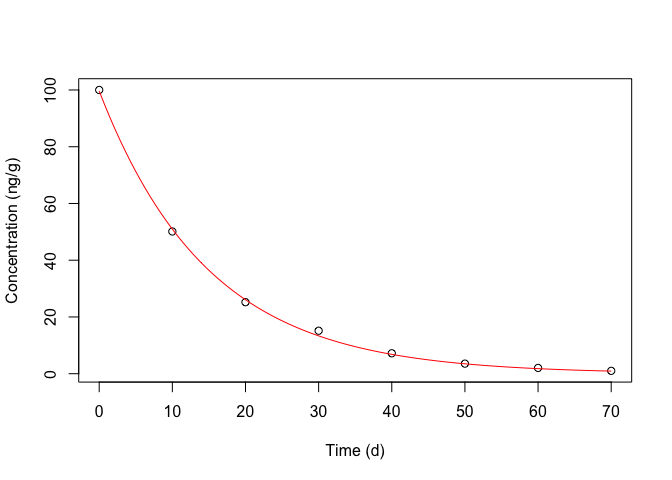
\includegraphics[width=0.9\linewidth]{_main_files/figure-latex/figName155-1} 

}

\caption{Degradation kinetic for metamitron in soil: symbols show the observed data, the red line shows the fitted equation}\label{fig:figName155}
\end{figure}

\hypertarget{approximate-f-test-for-lack-of-fit}{%
\subsection{Approximate F test for lack of fit}\label{approximate-f-test-for-lack-of-fit}}

If we have replicates, we can fit an ANOVA model and compare this latter model to the nonlinear regression model, as we have already shown in Chapter 13, for linear regression models (F test for lack of fit). With R, this test can be performed by using the \texttt{anova()} method and passing the two model objects as arguments. The box below shows that the null hypothesis of no lack of fit can be accepted.

\begin{Shaded}
\begin{Highlighting}[]
\NormalTok{modAov }\OtherTok{\textless{}{-}} \FunctionTok{lm}\NormalTok{(Conc }\SpecialCharTok{\textasciitilde{}} \FunctionTok{factor}\NormalTok{(Time), }\AttributeTok{data=}\NormalTok{dataset)}
\FunctionTok{anova}\NormalTok{(modNlin, modAov)}
\end{Highlighting}
\end{Shaded}

\begin{verbatim}
## Analysis of Variance Table
## 
## Model 1: Conc ~ A * exp(-k * Time)
## Model 2: Conc ~ factor(Time)
##   Res.Df Res.Sum Sq Df Sum Sq F value Pr(>F)
## 1     22     151.18                         
## 2     16     135.94  6 15.238  0.2989 0.9284
\end{verbatim}

\hypertarget{the-coefficient-of-determination-r2}{%
\subsection{\texorpdfstring{The coefficient of determination (R\textsuperscript{2})}{The coefficient of determination (R2)}}\label{the-coefficient-of-determination-r2}}

The R\textsuperscript{2} coefficient in nonlinear regression should not be used as a measure of goodness of fit, because it represents the ratio between the residual deviances for the model under comparison and for a model with the only intercept (see previous chapter). Some non-linear models do not have an intercept and, therefore, the R\textsuperscript{2} value is not meaningful and can also assume values outside the range from 0 to 1.

Such an argument can be, at least partly, overcame by using the \textbf{Pseudo R\textsuperscript{2}} (Schabenberger and Pierce, 2002), that is the proportion of variance explained by the regression effect:

\[R_a^2  = 1 - \frac{MSE}{MST}\]

where MSE is the residual mean square and MST is total mean square. For our example:

\vspace{12pt}

\begin{Shaded}
\begin{Highlighting}[]
\NormalTok{MSE }\OtherTok{\textless{}{-}} \FunctionTok{summary}\NormalTok{(modNlin)}\SpecialCharTok{$}\NormalTok{sigma }\SpecialCharTok{\^{}} \DecValTok{2}
\NormalTok{MST }\OtherTok{\textless{}{-}} \FunctionTok{var}\NormalTok{(dataset}\SpecialCharTok{$}\NormalTok{Conc)}
\DecValTok{1} \SpecialCharTok{{-}}\NormalTok{ MSE}\SpecialCharTok{/}\NormalTok{MST}
\end{Highlighting}
\end{Shaded}

\begin{verbatim}
## [1] 0.9936359
\end{verbatim}

Whenever necessary, The Pseudo-R\textsuperscript{2} value can be obtained by using the \texttt{R2nls()} function, in the `aomisc' package, as shown in the box below.

\vspace{12pt}

\begin{Shaded}
\begin{Highlighting}[]
\FunctionTok{R2nls}\NormalTok{(modNlin)}\SpecialCharTok{$}\NormalTok{PseudoR2}
\end{Highlighting}
\end{Shaded}

\begin{verbatim}
## [1] 0.9939126
\end{verbatim}

\hypertarget{stabilising-transformations-1}{%
\section{Stabilising transformations}\label{stabilising-transformations-1}}

In some cases, it may happen that the model does not fit the data (\textbf{lack of fit}) or that the residuals are not gaussian and homoscedastic. In the first case, we have to discard the model and select a new one, that fits better to the observed data.

In the other cases (heteroscedastic or non-normal residuals), similarly to linear regression, we should adopt some sort of stabilising transformations, possibly selected by using the Box-Cox method. However, nonlinear regression poses an additional issue, that we should keep into account. Indeed, in most cases, the parameters of nonlinear models are characterised by a clear biological meaning, such as, for example, the parameter \(a\) in the exponential equation above, that is the initial concentration value. If we transform the response into, e.g., its logarithm, the estimated \(a\) represents the logarithm of the initial concentration and its biological meaning is lost.

In order to avoid such a problem and obtain parameter estimates in their original scale, the `transform-both-sides' approach is feasible, where we use the Box-Cox family of transformations (see Chapter 8) to transform both the response and the model:

\[Y_i^\lambda  = f(X_i)^\lambda + \varepsilon_i\]

In order to use this technique in R, we can use the \texttt{boxcox.nls()} method in the `aomisc' package, that is very similar to the `boxcox()' method in the MASS package (see Chapter 8). The \texttt{boxcox.nls()} method returns the maximum likelihood value for \(\lambda\) with confidence intervals and a likelihood graph as a function of \(\lambda\) can also be obtained by using the argument `plotit = T'

\vspace{12pt}

\begin{Shaded}
\begin{Highlighting}[]
\NormalTok{bc }\OtherTok{\textless{}{-}} \FunctionTok{boxcox}\NormalTok{(modNlin)}
\NormalTok{bc}\SpecialCharTok{$}\NormalTok{lambda}
\end{Highlighting}
\end{Shaded}

\begin{verbatim}
## $lambda
## [1] 0.8
## 
## $ci
## [1] 0.5619080 0.9637162
\end{verbatim}

\begin{Shaded}
\begin{Highlighting}[]
\FunctionTok{boxcox}\NormalTok{(modNlin, }\AttributeTok{plotit =}\NormalTok{ T)}
\end{Highlighting}
\end{Shaded}

\begin{figure}

{\centering 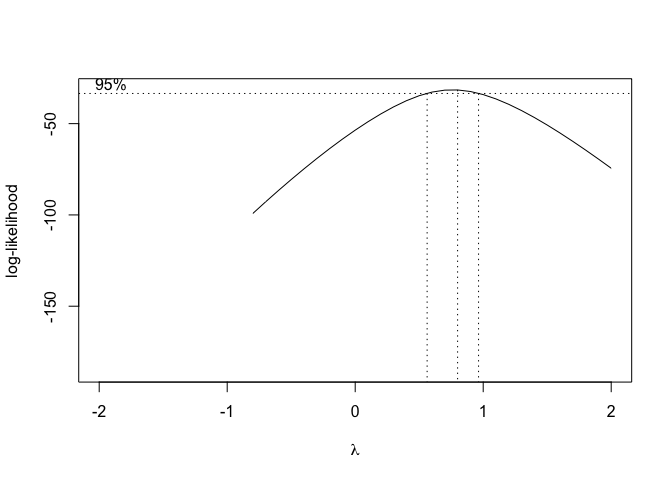
\includegraphics[width=0.9\linewidth]{_main_files/figure-latex/figName156-1} 

}

\caption{Selection of the 'lambda' value for the Box-Cox transformation of a nonlinear regression model}\label{fig:figName156}
\end{figure}

From Figure \ref{fig:figName156}, we see that the transformation is not required, although a value \(\lambda\) = 0.5 (square-root transformation; see previous chapter) might be used to maximise the likelihood of the data under the selected model. We can specify our favourite \(\lambda\) value and get the corresponding fit by using the same \texttt{boxcox.nsl()} function and passing an extra-argument, as shown in the box below.

\vspace{12pt}

\begin{Shaded}
\begin{Highlighting}[]
\NormalTok{modNlin3 }\OtherTok{\textless{}{-}} \FunctionTok{boxcox}\NormalTok{(modNlin, }\AttributeTok{lambda =} \FloatTok{0.5}\NormalTok{)}
\FunctionTok{summary}\NormalTok{(modNlin3)}
\end{Highlighting}
\end{Shaded}

\begin{verbatim}
## 
## Formula: bcFct1(Conc) ~ bcFct2(A * exp(-k * Time))
## 
## Parameters:
##    Estimate Std. Error t value Pr(>|t|)    
## A 99.532761   4.625343   21.52 2.87e-16 ***
## k  0.067068   0.002749   24.40  < 2e-16 ***
## ---
## Signif. codes:  
## 0 '***' 0.001 '**' 0.01 '*' 0.05 '.' 0.1 ' ' 1
## 
## Residual standard error: 0.9196 on 22 degrees of freedom
## 
## Number of iterations to convergence: 1 
## Achieved convergence tolerance: 7.541e-06
\end{verbatim}

We see that, in spite of the stabilising transformation, the estimated parameters have not lost their measurement unit.

\hypertarget{making-predictions-1}{%
\section{Making predictions}\label{making-predictions-1}}

As shown for linear regression in Chapter 13, every fitted model can be used to make predictions, i.e.~to calculate the response for a given X-value or to calculate the X-value corresponding to a given response.

Analogously to linear regression, we could make predictions by using the \texttt{predict()} method, although, for nonlinear regression objects, this method does not return standard errors. Therefore, we can use the \texttt{gnlht()} function in the `aomisc' package, which requires the following arguments:

\begin{enumerate}
\def\labelenumi{\arabic{enumi}.}
\tightlist
\item
  a list of functions containing model parameters (with the same names as the fitted model) and, possibly, some other parameters
\item
  if the previous function contain further parameters with respect to the fitted model, their values need to be given in a data frame as an extra-argument
\end{enumerate}

In the box below we make predictions for the response at 5, 10 and 15 days after the beginning of the experiment.

\vspace{12pt}

\begin{Shaded}
\begin{Highlighting}[]
\NormalTok{func }\OtherTok{\textless{}{-}} \FunctionTok{list}\NormalTok{(}\SpecialCharTok{\textasciitilde{}}\NormalTok{A }\SpecialCharTok{*} \FunctionTok{exp}\NormalTok{(}\SpecialCharTok{{-}}\NormalTok{k }\SpecialCharTok{*}\NormalTok{ time))}
\NormalTok{const }\OtherTok{\textless{}{-}} \FunctionTok{data.frame}\NormalTok{(}\AttributeTok{time =} \FunctionTok{c}\NormalTok{(}\DecValTok{5}\NormalTok{, }\DecValTok{10}\NormalTok{, }\DecValTok{15}\NormalTok{)) }
\FunctionTok{gnlht}\NormalTok{(modNlin, func,  const)}
\end{Highlighting}
\end{Shaded}

\begin{verbatim}
##                 Form time Estimate        SE  t-value
## 1 A * exp(-k * time)    5 71.25873 0.9505532 74.96553
## 2 A * exp(-k * time)   10 50.96413 0.9100611 56.00078
## 3 A * exp(-k * time)   15 36.44947 0.9205315 39.59611
##        p-value
## 1 5.340741e-28
## 2 3.163518e-25
## 3 6.029672e-22
\end{verbatim}

The same method can be used to make inverse predictions. In our case, the inverse function is:

\[X = - \frac{log \left( \frac{Y}{A} \right)}{k}\]

We can calculate the times required for the concentration to drop to, e.g., 10 and 20 mg/g by using the code in the following box.

\vspace{12pt}

\begin{Shaded}
\begin{Highlighting}[]
\NormalTok{func }\OtherTok{\textless{}{-}} \FunctionTok{list}\NormalTok{(}\SpecialCharTok{\textasciitilde{}} \SpecialCharTok{{-}}\NormalTok{(}\FunctionTok{log}\NormalTok{(Conc}\SpecialCharTok{/}\NormalTok{A)}\SpecialCharTok{/}\NormalTok{k))}
\NormalTok{const }\OtherTok{\textless{}{-}} \FunctionTok{data.frame}\NormalTok{(}\AttributeTok{Conc =} \FunctionTok{c}\NormalTok{(}\DecValTok{10}\NormalTok{, }\DecValTok{20}\NormalTok{)) }
\FunctionTok{gnlht}\NormalTok{(modNlin, func,  const)}
\end{Highlighting}
\end{Shaded}

\begin{verbatim}
##               Form Conc Estimate        SE  t-value
## 1 -(log(Conc/A)/k)   10 34.29237 0.8871429 38.65484
## 2 -(log(Conc/A)/k)   20 23.95291 0.6065930 39.48761
##        p-value
## 1 1.016347e-21
## 2 6.399715e-22
\end{verbatim}

In the same fashion, we can calculate the half-life (i.e.~the time required for the concentration to drop to half of the initial value), by considering that:

\[t_{1/2} = - \frac{ \log \left( {\frac{1}{2}} \right) }{k}\]

The code is::

\vspace{12pt}

\begin{Shaded}
\begin{Highlighting}[]
\NormalTok{func }\OtherTok{\textless{}{-}} \FunctionTok{list}\NormalTok{(}\SpecialCharTok{\textasciitilde{}} \SpecialCharTok{{-}}\NormalTok{(}\FunctionTok{log}\NormalTok{(}\FloatTok{0.5}\NormalTok{)}\SpecialCharTok{/}\NormalTok{k))}
\FunctionTok{gnlht}\NormalTok{(modNlin, func)}
\end{Highlighting}
\end{Shaded}

\begin{verbatim}
##            Form Estimate       SE t-value      p-value
## 1 -(log(0.5)/k) 10.33945 0.291017 35.5287 6.318214e-21
\end{verbatim}

The `gnlht()' function provides standard errors based on the delta method, which we have already introduced in a previous chapter.

\begin{center}\rule{0.5\linewidth}{0.5pt}\end{center}

\hypertarget{further-readings-11}{%
\section{Further readings}\label{further-readings-11}}

\begin{enumerate}
\def\labelenumi{\arabic{enumi}.}
\tightlist
\item
  Bates, D.M., Watts, D.G., 1988. Nonlinear regression analysis \& its applications. John Wiley \& Sons, Inc., Books.
\item
  Bolker, B.M., 2008. Ecological models and data in R. Princeton University Press, Books.
\item
  Carroll, R.J., Ruppert, D., 1988. Transformation and weighting in regression. Chapman and Hall, Books.
\item
  Ratkowsky, D.A., 1990. Handbook of nonlinear regression models. Marcel Dekker Inc., Books.
\item
  Ritz, C., Streibig, J.C., 2008. Nonlinear regression with R. Springer-Verlag New York Inc., Books.
\item
  Schabenberger, O., Pierce, F.J., 2002. Contemporary statistical models for the plant and soil sciences. Taylor \& Francis, CRC Press
\end{enumerate}

\hypertarget{exercises}{%
\chapter{Exercises}\label{exercises}}

Placeholder

\hypertarget{chapter-3}{%
\section{Chapter 3}\label{chapter-3}}

\hypertarget{exercise-1}{%
\subsection{Exercise 1}\label{exercise-1}}

\hypertarget{exercise-2}{%
\subsection{Exercise 2}\label{exercise-2}}

\hypertarget{exercise-3}{%
\subsection{Exercise 3}\label{exercise-3}}

\hypertarget{chapter-4}{%
\section{Chapter 4}\label{chapter-4}}

\hypertarget{exercise-1-1}{%
\subsection{Exercise 1}\label{exercise-1-1}}

\hypertarget{exercise-2-1}{%
\subsection{Exercise 2}\label{exercise-2-1}}

\hypertarget{exercise-3-1}{%
\subsection{Exercise 3}\label{exercise-3-1}}

\hypertarget{exercise-4}{%
\subsection{Exercise 4}\label{exercise-4}}

\hypertarget{exercise-5}{%
\subsection{Exercise 5}\label{exercise-5}}

\hypertarget{chapter-5}{%
\section{Chapter 5}\label{chapter-5}}

\hypertarget{exercise-1-2}{%
\subsection{Exercise 1}\label{exercise-1-2}}

\hypertarget{exercise-2-2}{%
\subsection{Exercise 2}\label{exercise-2-2}}

\hypertarget{exercise-3-2}{%
\subsection{Exercise 3}\label{exercise-3-2}}

\hypertarget{exercise-4-1}{%
\subsection{Exercise 4}\label{exercise-4-1}}

\hypertarget{chapter-6}{%
\section{Chapter 6}\label{chapter-6}}

\hypertarget{exercise-1-3}{%
\subsection{Exercise 1}\label{exercise-1-3}}

\hypertarget{exercise-2-3}{%
\subsection{Exercise 2}\label{exercise-2-3}}

\hypertarget{exercise-3-3}{%
\subsection{Exercise 3}\label{exercise-3-3}}

\hypertarget{exercise-4-2}{%
\subsection{Exercise 4}\label{exercise-4-2}}

\hypertarget{exercise-5-1}{%
\subsection{Exercise 5}\label{exercise-5-1}}

\hypertarget{exercise-6}{%
\subsection{Exercise 6}\label{exercise-6}}

\hypertarget{exercise-7}{%
\subsection{Exercise 7}\label{exercise-7}}

\hypertarget{chapters-7-to-9}{%
\section{Chapters 7 to 9}\label{chapters-7-to-9}}

\hypertarget{exercise-1-4}{%
\subsection{Exercise 1}\label{exercise-1-4}}

\hypertarget{exercise-2-4}{%
\subsection{Exercise 2}\label{exercise-2-4}}

\hypertarget{exercise-3-4}{%
\subsection{Exercise 3}\label{exercise-3-4}}

\hypertarget{exercise-4-3}{%
\subsection{Exercise 4}\label{exercise-4-3}}

\hypertarget{chapter-10}{%
\section{Chapter 10}\label{chapter-10}}

\hypertarget{exercise-1-5}{%
\subsection{Exercise 1}\label{exercise-1-5}}

\hypertarget{exercise-2-5}{%
\subsection{Exercise 2}\label{exercise-2-5}}

\hypertarget{exercise-3-5}{%
\subsection{Exercise 3}\label{exercise-3-5}}

\hypertarget{chapters-11-and-12}{%
\section{Chapters 11 and 12}\label{chapters-11-and-12}}

\hypertarget{exercise-1-6}{%
\subsection{Exercise 1}\label{exercise-1-6}}

\hypertarget{exercise-2-6}{%
\subsection{Exercise 2}\label{exercise-2-6}}

\hypertarget{exercise-3-6}{%
\subsection{Exercise 3}\label{exercise-3-6}}

\hypertarget{exercise-4-4}{%
\subsection{Exercise 4}\label{exercise-4-4}}

\hypertarget{exercise-5-2}{%
\subsection{Exercise 5}\label{exercise-5-2}}

\hypertarget{exercise-6-1}{%
\subsection{Exercise 6}\label{exercise-6-1}}

\hypertarget{chapter-13}{%
\section{Chapter 13}\label{chapter-13}}

\hypertarget{exercise-1-7}{%
\subsection{Exercise 1}\label{exercise-1-7}}

\hypertarget{exercise-2-7}{%
\subsection{Exercise 2}\label{exercise-2-7}}

\hypertarget{chapter-14}{%
\section{Chapter 14}\label{chapter-14}}

\hypertarget{exercise-1-8}{%
\subsection{Exercise 1}\label{exercise-1-8}}

\hypertarget{exercise-2-8}{%
\subsection{Exercise 2}\label{exercise-2-8}}

\hypertarget{exercise-3-7}{%
\subsection{Exercise 3}\label{exercise-3-7}}

\hypertarget{exercise-4-5}{%
\subsection{Exercise 4}\label{exercise-4-5}}

\hypertarget{exercise-5-3}{%
\subsection{Exercise 5}\label{exercise-5-3}}

\hypertarget{exercise-6-2}{%
\subsection{Exercise 6}\label{exercise-6-2}}

\hypertarget{exercise-7-1}{%
\subsection{Exercise 7}\label{exercise-7-1}}

\hypertarget{appendix-a-very-gentle-introduction-to-r}{%
\chapter{APPENDIX: A very gentle introduction to R}\label{appendix-a-very-gentle-introduction-to-r}}

Placeholder

\hypertarget{what-is-r}{%
\section{What is R?}\label{what-is-r}}

\hypertarget{installing-r-and-moving-the-first-steps}{%
\section{Installing R and moving the first steps}\label{installing-r-and-moving-the-first-steps}}

\hypertarget{assignments}{%
\section{Assignments}\label{assignments}}

\hypertarget{data-types-and-data-objects}{%
\section{Data types and data objects}\label{data-types-and-data-objects}}

\hypertarget{matrices}{%
\section{Matrices}\label{matrices}}

\hypertarget{dataframes}{%
\section{Dataframes}\label{dataframes}}

\hypertarget{working-with-objects}{%
\section{Working with objects}\label{working-with-objects}}

\hypertarget{expressions-functions-and-arguments}{%
\section{Expressions, functions and arguments}\label{expressions-functions-and-arguments}}

\hypertarget{a-few-useful-functions}{%
\section{A few useful functions}\label{a-few-useful-functions}}

\hypertarget{extractors}{%
\section{Extractors}\label{extractors}}

\hypertarget{reading-external-data}{%
\section{Reading external data}\label{reading-external-data}}

\hypertarget{simple-r-graphics}{%
\section{Simple R graphics}\label{simple-r-graphics}}

\hypertarget{further-readings-12}{%
\section{Further readings}\label{further-readings-12}}


\end{document}
